\chapter{Implémentation}
Les structures et fonctions demandées dans le sujet ont été implémentées, avec quelques spécificités selon la compréhension du sujet. Par exemple, certains vérifications ont été ajoutées (vérification qu'un arbre ou qu'un n\oe ud n'est pas \lstinline{NULL}). De plus, un mot est caractérisé par son numéro de ligne, son numéro de phrase et son ordre. \textbf{\color{red}Nous avons implémenté cela de telle sorte que l'ordre corresponde à l'ordre dans la phrase, et non à l'ordre dans la ligne.}

\section{Programme principal}
Le programme principal affiche à l'utilisateur un menu qui lui donne le choix parmi \textbf{7 possibilités} :
\begin{enumerate}
  \item Créer un ABR
  \item Charger un fichier dans l'ABR
  \item Afficher les caractéristiques de l'ABR
  \item Afficher tous les mots distincts par ordre alphabétique
  \item Rechercher un mot
  \item Afficher les phrases contenant deux mots
  \item Quitter le programme
\end{enumerate}
L'utilisateur tape au clavier le numéro de son choix. Un \lstinline{switch} permet d'effectuer les actions correspondantes à l'entrée clavier.
\textcode{main.c}
\begin{lstlisting}
// ...
afficherMenu();
while((inputUser = getchar()) != '7') {
  // ...
  switch(inputUser) {
    case '1':
        // ...
        break;
    case '2':
        // ...
        break;
    case '3':
        // ...
        break;
    case '4':
        // ...
        break;
    case '5':
        // ...
        break;
    case '6':
        // ...
        break;
    default:
        printf("Mauvaise entrée. Veuillez taper 1, 2, 3, 4, 5, 6 ou 7.\n");
        continue; // On recommence la boucle while
  }
  // ...
  afficherMenu();
}
// ...
\end{lstlisting}
Une boucle \lstinline{while} permet d'afficher à nouveau le menu après être sorti du \lstinline{switch}. L'invariant de boucle est \textbf{\lstinline{(inputUser = getchar()) != '7'}}.

\section{Autres fichiers}
Les autres fonctions ont été écrites comme demandées.. Pour l'affichage de l'arbre, l'algorithme de \textbf{parcours infixe} vu en cours a été implémenté. Il en va de même pour les algorithmes \textbf{d'ajout d'un n\oe ud à l'arbre} en tenant compte de l'ordre des mots, de \textbf{recherche d'un n\oe ud dans l'abre} et pour l'algorithme qui \textbf{retourne la hauteur d'un arbre}.

\subsection{Ajouts par rapport au sujet}
\subsubsection{\lstinline{struct mot} et \lstinline{struct phrase}}
Par rapport à ce qui a été demandé, nous avons choisi d'ajouter deux structures (deux listes chaînées) :
\textcode{outils.h}
\begin{lstlisting}
typedef struct mot {
    char* mot;
    struct mot *suivant;
} Mot;

typedef struct phrase {
    int numero;
    Mot *debut;
    struct phrase *suivante;
} Phrase;
\end{lstlisting}
Ces deux listes chaînées sont remplies au fur et à mesure que l'on \textit{parse} (parcourt) le fichier texte lu, grâce à plusieurs \textbf{fonctions que nous avons ajoutées} dans les fichiers \textbf{outils.c} et \textbf{outils.h}. Ainsi, lorsque l'utilisateur choisi deux mots (option 6 du menu), grâce à la fonction \lstinline{NoeudABR *rechercher_noeud(ArbreBR *arbre, char *mot)} on peut aisément retrouver les numéros de phrase où les deux mots sont présents. Puis l'affichage de la ou des phrases est rendu très simple grâce à nos deux listes chaînées.
\textcode{outils.c}
\begin{lstlisting}
void afficher_phrase(Phrase *phrase, int numero) { // La phrase 1 est passée en paramètre, elle pointe sur la 2, qui pointe sur la 3, etc
  while(phrase != NULL) {
    if (phrase->numero == numero) { // Si c'est la bonne phrase, on l'affiche
      Mot *mot = phrase->debut;
      while (mot != NULL) {
        printf("%s ",mot->mot);
        mot = mot->suivant;
      }
    }
    phrase = phrase->suivante;
  }
  printf(".\n");
}
\end{lstlisting}

\subsubsection{Autres ajouts}
Dans \textbf{arbre.h} et \textbf{arbre.c}, nous avons ajouté d'autres fonctions, dont le nom est suffisamment évoquant pour ne pas être expliquéees :
\begin{itemize}
  \item \lstinline{void parcours_infixe(NoeudABR *n)}
  \item \lstinline{void supprimerNoeud(NoeudABR *noeud)}
  \item \lstinline{int max (int a, int b)}
  \item \lstinline{int getHauteur(NoeudABR *noeud)}
  \item \lstinline{int isEquilibre(NoeudABR *n)}
\end{itemize}

Quant aux fichiers \textbf{liste.h} et \textbf{liste.c}, seule la fonction \lstinline{void supprimerPosition(Position *pos)} a été ajoutée. Elle supprime toutes les positions d'un mot.

\section{Difficulté rencontrée}
La difficulté majeure rencontrée dans ce TP a été l'implémentation de la fonction qui lit un fichier et stocke chaque mot dans un n\oe ud de l'arbre. Il faut en effet être capable de détecter la fin d'un mot, lorsque l'on rencontre soit un espace, soit un point, soit un retour à la ligne. De plus, si je rencontre un espace ou un retour à la ligne alors que le caractère précédent était un point, il ne faut pas ajouter de mot. Il fallait également prendre en compte le fait qu'un fichier ne finit pas nécessairement par un point. Enfin, sur Windows, le caractère de saut de ligne est \textbf{\lstinline{\\r\\n}} alors que sur les systèmes UNIX c'est \textbf{\lstinline{\\n}}. Il fallait donc prendre en considération tous ces aspects.

\medskip

\noindent\fbox{\color{red}%
\parbox{0.99\textwidth}{
\textbf{ATTENTION : L'ordre d'un mot correspond à l'ordre dans la phrase, et non à l'ordre dans la ligne.}
}}

\medskip

Au final, la fonction est plutôt conséquente :
\textcode{outils.c}
\begin{lstlisting}
int charger_fichier(ArbreBR *arbre, char *filename) {
    if (arbre == NULL)
        return 0;

    FILE *fp;
    int c, c_old;

    int ligne = 1, ordre = 1, phrase = 1;
    char *mot = (char*) malloc(sizeof(char)*26);
    int counter = 0, total = 0;

    fp = fopen(filename, "r");
    if (fp == NULL) {
        perror("Le fichier ne peut pas être ouvert.");
        return 0;
    }
    do {
        c_old = c;
        c = fgetc(fp);
        if (feof(fp)) // END OF FILE
            break;

        if (c == EOF || c == '\n') {
            if (c_old != '.' && c_old != ' ') {
                total++;
                mot[counter] = 0;
                saveWord(arbre,mot,ligne,ordre,phrase);
                ordre++;
            }
            ligne++;

            counter = 0;
            mot = (char*) malloc(sizeof(char)*26);
        }
        else if (c == ' ') {
            if (c_old != '.') {
                total++;
                mot[counter] = 0;
                saveWord(arbre,mot,ligne,ordre,phrase);
                ordre++;
            }

            counter = 0;
            mot = (char*) malloc(sizeof(char)*26);
        }
        else if (c == '.') {
            mot[counter] = 0;
            saveWord(arbre,mot,ligne,ordre,phrase);
            counter = 0;
            total++;
            ordre = 1;
            phrase++;
        }
        else {
            if (c == '\r') {
                c = c_old;
                continue; // WINDOWS
            }
            mot[counter] = c;
            counter++;
        }
    }while(1);

    if (c_old != '.' && c_old != ' ' && c_old != '\n') {
        saveWord(arbre,mot,ligne,ordre,phrase);
        total++;
    }

    fclose(fp);
    return total;
}
\end{lstlisting}

\chapter{Capture d'écran}
\noindent Voici un aperçu de notre programme :
\begin{figure}[!h]
   \centering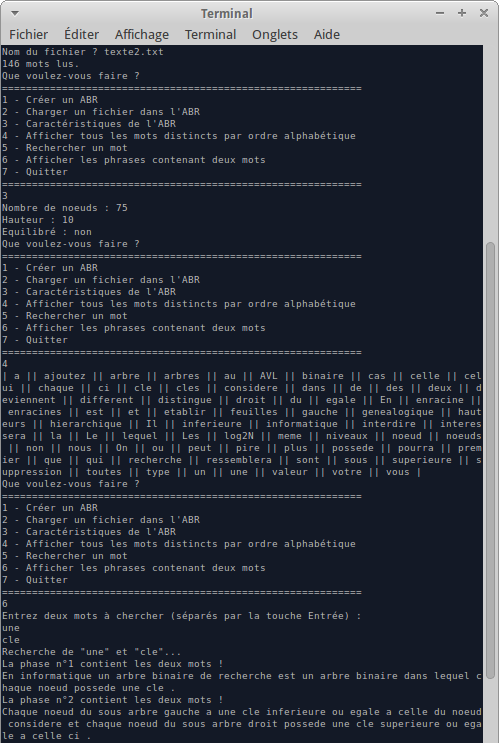
\includegraphics[width=0.8\textwidth]{sample.png}
   \caption{L'utilisateur a choisi 1, 2, 3, 4 et enfin 6 dans le menu d'options}
\end{figure}